\chapter{La memoria cache dei principali Web Browser}

La memoria cache, propria di ogni browser, risiede all'interno di una directory nel disco. 

Le modalità con le quali le informazioni presenti in cache vengono mantenute, la struttura della directory, i vari file che la compongono ed i collegamenti fra di essi variano fra i vari browser presi in esame. 

Il grafico mostra le percentuali di diffusione fra gli utenti dei principali browser, in un periodo di sei mesi.

\begin{figure}[htpb]
	\begin{center}
		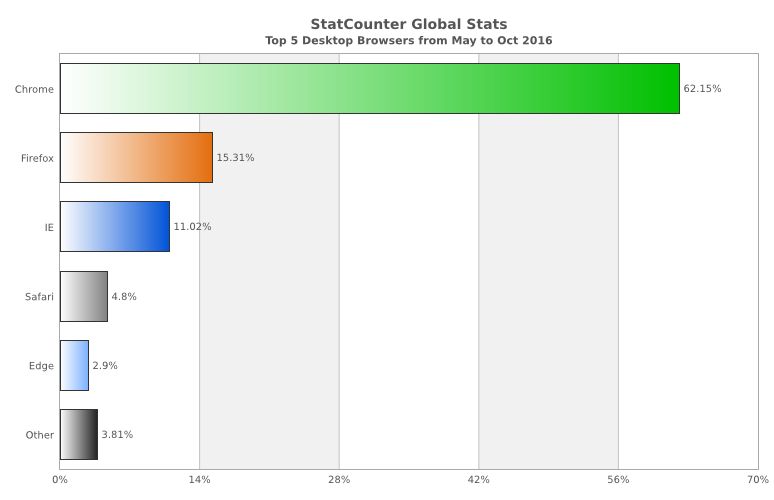
\includegraphics[scale=0.55]{StatCounter_browser_201605_201610_bar.png}
	\end{center}
\caption[Popolarità dei web browsers mag 2016 - ott 2016]{Popolarità dei web browser mag 2016 - ott 2016 \footnotemark}
\end{figure}
\footnotetext{\url{http://gs.statcounter.com/\#desktop-browser-ww-monthly-201605-201610-bar}} 

\section{Google Chrome}

Lanciato nel 2008 da parte di Google sulla base del progetto open source \textbf{Chromium}, il browser Google Chrome risulta esserne la versione compilata e distribuita da Google.
Al suo rilascio, nel settembre 2008, è stato reso pubblico anche il codice sorgente alla base di Chromium, con lo scopo di utilizzarlo come \textit{core} open source dell'applicazione, sottoponendolo nel frattempo alla revisione del codice da parte della comunità \footnote{\url{http://www.google.com/intl/it/chrome/timemachine/}}. 
Rispetto a Chromium, il cui sviluppo ed i suoi rilasci sono gestiti dalla comunità di sviluppatori, Google Chrome viene distribuito ed aggiornato da Google stessa secondo una propria tabella di marcia.
Le differenze fra i due browser si notano principalmente nella natura \textit{open source} o \textit{closed source}, con Google Chrome che annovera anche estensioni e plugin closed source al contrario di Chromium. \footnote{\url{https://chromium.googlesource.com/chromium/src/+/master/docs/chromium_browser_vs_google_chrome.md}} \nocite{Chromium}

La struttura e gestione della memoria cache risulta essere uguale fra i due browser.

\subsection{Struttura della memoria cache}

I file componenti la cache sono mantenuti in una cartella sul disco la cui locazione di default dipende dal sistema operativo in uso. Per sistemi Windows si ha: 

\begin{itemize}
	\item{\texttt{C:\textbackslash Users\textbackslash\%Username\%\textbackslash AppData\textbackslash Local\textbackslash Google\textbackslash Chrome\textbackslash User Data\textbackslash Default\textbackslash Cache}}
\end{itemize}

Nella cartella della cache sono presenti almeno 5 files: un file \textbf{\textit{index}} e 4 \textbf{\textit{data\_\# \footnote{Il \# indica un numero progressivo a partire da 0}}}. Altri file opzionali, detti \textbf{\textit{separate file}}, contengono informazioni la cui dimensione è maggiore di quella massima consentita per i file data\_\#.

\begin{figure}[h]
	\centering
	\begin{minipage}[c]{0.7\textwidth}
		\dirtree{%
			.1 \textit{\textbf{GOOGLE CHROME CACHE FOLDER}}.
			.2 \textit{Index file} \DTcomment{//Sempre presente}.
			.2 \textit{Block file data\_0} \DTcomment{//Sempre presente}.
			.2 \textit{Block file data\_1} \DTcomment{//Sempre presente}.
			.2 \textit{Block file data\_2} \DTcomment{//Sempre presente}.
			.2 \textit{Block file data\_3} \DTcomment{//Sempre presente}.
			.2 \textit{Separate file f\_\#\#\#\#\#\#}  \DTcomment{//Opzionale}.
			.2 \vdots.
			.2 \vdots.
			.2 \vdots.
			.2 \textit{Separate file f\_\#\#\#\#\#\#} \DTcomment{//Opzionale}.
		} 
	\end{minipage}
	\caption{Chrome: struttura della cartella \textbf{\textit{cache}}}
\end{figure}

\subsection{Struttura dei file}
Il file \textbf{\textit{index}} si presenta come una struttura formata da un \textit{index header} e da una \textit{tabella hash}. Il numero di elementi presenti nella tabella è definito dal parametro \textit{table\_len} presente nell'header. 

Qui gli elementi sono rappresentati secondo il formato \textbf{\textit{little endian}}. Ognuno di essi esprime il nome della risorsa (\textbf{\textit{key}}) e l'indirizzo in cache che la contiene. Convertendo in formato binario a 32 bit ed analizzandone le varie sezioni si ottiene la locazione esatta (file e posizione al suo interno) di una risorsa che presenta lo stesso \textit{hash}.

\begin{savenotes}
	\begin{table}[H]
		\rowcolors{2}{lightgray}{white}
		\begin{center}
			\resizebox{0.65\textwidth}{!}{
			\begin{tabular}{ccc}
				\textbf{Offset} &\textbf{Size} &\textbf{Description}\\  \hline
				If file type is 0 (Separate file) & &\\
				0.0 &28 bits &File number \footnote{Valore di \# in f\_\#\#\#\#\#\#}\\
				Else \\
				0.0 &16 bits &Block number \\
				2.0 &8 bits &File number (or file selector) \footnote{Valore di \# in data\_\#}\\
				3.0 &2 bits &Block size \footnote{Numero di blocchi contigui: 0 rappresenta 1 blocco, 3 rappresenta 4 blocchi}  \\
				3.2 &2 bits &Reserved\\
				Common  & &\\
				3.4 &3 bits &File type\\
				3.7 &1 bits &Initialized flag\\			
			\end{tabular}}
		\end{center}
		\caption{Chrome: struttura di un indirizzo cache}
	\end{table}
\end{savenotes}

\begin{table}[H]
	\rowcolors{2}{lightgray}{white}
	\begin{center}
		\resizebox{0.85\textwidth}{!}{
			\begin{tabular}{ccccccc}
				&Init &File type &Reserved &Contiguous blocks &File number  &Block number \\ \hline
				Binary &1 &010 &00 &00 &0000 0001 &0000 0000 0000 0011 \\
				Integer &1 &2 &0 &0 &1 &3 
			\end{tabular}}
	\end{center}
	\caption{Chrome: esempio di un indirizzo cache}
\end{table}

Interpretando il campo \textit{file type} nell'indirizzo si ottiene il file contenente la risorsa.
	
\begin{table}[H]
	\rowcolors{2}{lightgray}{white}
	\begin{center}
		\resizebox{0.6\textwidth}{!}{
		\begin{tabular}{ccc}
			\textbf{Binary} &\textbf{Integer} &\textbf{Interpretation}\\  \hline
			000 & 0 &Separate file\\
			001 & 1 &Ranking (36 byte block file)\\
			010 & 2 &256 byte block file\\
			011 & 3 &1 KByte block file\\
			100 & 4 &4 KByte block file\\
		\end{tabular}}
	\end{center}
	\caption{Chrome: tipi di file presenti nella cache}
\end{table}


I data\_\# file, indicati anche come \textbf{\textit{block file}}, sono costituiti da un \textit{header} seguito da un numero variabile (con un massimo di 64000) di \textit{blocchi} aventi dimensione fissa. Se venisse richiesta la presenza di ulteriori blocchi della stessa dimensione, un nuovo file data\_\# viene creato e collegato al precedente mediante il campo \textit{next\_file} presente nell'header. 
All'interno dei block file le informazioni vengono memorizzate utilizzando un massimo di 4 blocchi consecutivi. Se la dimensione dell'informazione da memorizzare dovesse superare quella di 4 blocchi consecutivi, questa viene memorizzata in un data file\_\# con blocchi di dimensioni maggiori. Se nessun data\_\# file è in grado di poter contenere l'informazione, questa viene salvata all'interno di \textbf{\textit{separate file}}
\newline

I \textbf{\textit{separate file}} (\textit{f\_\#\#\#\#\#\#}) memorizzano le informazioni di dimensioni maggiori di 16 KByte. 
Il loro nome è espresso nella forma \textit{f\_} seguito da un numero esadecimale progressivo di 6 cifre. 
Questo tipo di file non presenta header ma contiene solamente dati.
\newline

Sia le risorse di dimensioni fino a 16 KByte nei \textit{data\_\# file}, sia quelle di dimensioni maggiori che risiedono nei \textit{f\_\#\#\#\#\#\#}, sono memorizzate in formato \textbf{\textit{gzip}}. 
\clearpage

\begin{figure}[htpb]
	\begin{center}
		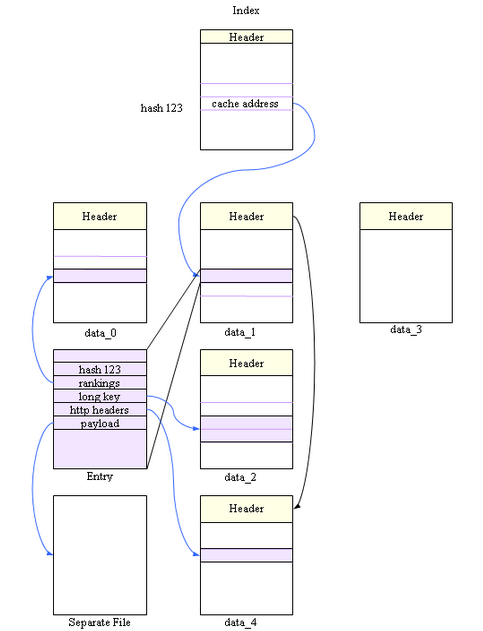
\includegraphics[scale=0.8]{Chrome_cache_overview.png}
	\end{center}
	\caption[Chrome: diagramma della cache]{Chrome: diagramma della cache \footnotemark}
\end{figure}
\footnotetext{\url{https://www.chromium.org/developers/design-documents/network-stack/disk-cache}}

Questo tipo di implementazione della memoria cache è valido per le versioni 1 e 2. Attualmente è in corso di sviluppo una nuova versione (v3) che renderà valido il modello di cache appena descritto solo per file salvati nelle versioni 1 e 2 \footnote{\url{https://www.chromium.org/developers/design-documents/network-stack/disk-cache/disk-cache-v3}}.
\clearpage

\section{Mozilla Firefox}

La fondazione Mozilla è un'organizzazione senza scopo di lucro con la missione di promuovere un Internet ``aperto ed accessibile a tutti''. \footnote{\url{https://www.mozilla.org/it/mission/}} 
Per questo sviluppa e rilascia \textbf{\textit{Firefox}}, un browser che propone fra le sue caratteristiche principali quella della sicurezza e della privacy durante la navigazione. \footnote{\url{https://www.mozilla.org/it/firefox/desktop/}}

Il progetto Mozilla fu lanciato il 31 Marzo 1998 con il rilascio in versione gratuita del codice sorgente del browser ``Netscape'' \footnote{\url{https://www.mozilla.org/en-US/about/history/details/}}. Supportato e sviluppato da una comunità indipendente, ne viene considerato il suo successore. Dal suo primo rilascio nel 2004 si è rivelato uno dei browser più apprezzati, rimanendo tuttora stabilmente tra quelli più utilizzati. 

\subsection{Struttura della memoria cache}

A partire dalla versione 32 del browser Firefox(settembre 2014 \footnote{\url{https://www.mozilla.org/en-US/firefox/32.0/releasenotes/}}), Mozilla ha introdotto un nuovo formato di cache per il proprio browser. \`E possibile trovare la directory contenente la cache alla locazione (per sistemi Windows):

\begin{itemize}
	\item{\texttt{C:\textbackslash Users\textbackslash\%Username\%\textbackslash AppData\textbackslash Local\textbackslash Mozilla\textbackslash Firefox\textbackslash Profiles\\\textbackslash random \footnote{Sequenza di 8 caratteri alfanumerici causali}.default\textbackslash Cache}}
\end{itemize}

All'interno di questa locazione si trovano varie sottocartelle in uso dal browser, compresa la cartella \textbf{\textit{cache2}} che contiene i file interessati. Scorrendo gli elementi presenti si trova un file \textbf{\textit{index}} al cui interno sono presenti record per ogni file presente nella cache. Le risorse vere e proprie, puntate dai record del file index si trovano in una sottocartella \textbf{\textit{entries}}.

\begin{figure}[h]
	\centering
	\begin{minipage}[c]{0.7\textwidth}
		\dirtree{%
			.1 \textit{\textbf{MOZILLA FIREFOX CACHE2 FOLDER}}.
			.2 \textit{Index File}.
			.2 \textit{Index.log File}.
			.2 \textit{Doomed folder}.
			.2 \textit{Entries folder}.
			.3 \textit{Entry}.
			.3 \vdots.
			.3 \vdots.
			.3 \vdots.
			.3 \textit{Entry}.
	} 
	\end{minipage}
	\caption{Firefox: struttura della cartella \textit{cache2}}
\end{figure}

\subsection{Struttura dei file}

Il file \textbf{\textit{index}} si presenta come una struttura formata da un \textit{header} e da una \textit{tabella hash} contenente i record che puntano alle \textit{entries} nella cartella \textbf{\textit{entries}}. \nocite{Habben}

I record nella tabella hash sono rappresentati secondo il formato \textbf{\textit{big endian}} ed indicano una risorsa contenuta all'interno di uno dei file nella cartella entries. 
\clearpage

Ogni record ha dimensione di 36 byte ed è così formato:


\begin{table}[H]
	\rowcolors{2}{lightgray}{white}
	\begin{center}
		\resizebox{0.7\textwidth}{!}{
			\begin{tabular}{cccc}
				\textbf{Offset} &\textbf{Size} &\textbf{Type} &\textbf{Description}\\  \hline
				0 &20 &SHA1 &Hash Of URL\\
				20 &4 &BE integer &Frequency\\
				24 &4 &BE Unix date &Expiration date\\
				28 &4 &BE integer &AppId \\
				32 &1 &Byte &Flags\\
				33 &3 &BE integer &File size \\
			\end{tabular}}
		\end{center}
		\caption{Firefox: struttura di un indirizzo cache}
\end{table}

\begin{table}[H]
	\begin{center}
		\resizebox{0.9\textwidth}{!}{
			\begin{tabular}{cccccc}
				Hash &Frequency &Exp date (Unix) &AppId &Flags  &File size \\ \hline
				2BD1F3E105AFF6A7CBFB &1025038823 &1481233511 &0 &128 &99 \\
				14955D5FA38873035CB5
			\end{tabular}}
		\end{center}
		\caption{Firefox: esempio di un indirizzo cache}
	\end{table}

I primi 20 byte rappresentano l'hash SHA1 dell'url della risorsa ed è con questo che vengono nominati i file all'interno della cartella \textit{entries}.

Questi file non presentano header ed il loro contenuto, rappresentato in formato \textbf{\textit{big endian}}, comincia a partire dalla prima locazione.
Alla fine del contenuto si trovano i metadati provenienti dal server web, come ad esempio l'header HTTP. Per conoscerne l'esatta posizione bisogna leggere gli ultimi 4 byte del file.
A partire dalla locazione indicata da questi si trovano in ordine 4 byte rappresentanti l'hash del contenuto del file, seguiti da porzioni di 2 byte dell'hash per ogni blocco da 256 KByte in cui può essere diviso il file.  
Dividendo la dimensione del file (in byte) per la dimensione del blocco (in byte) e arrotondando per eccesso in caso di resto della divisione, si ottiene il numero di blocchi presenti all'interno del file,  
A questo punto si moltiplica il numero di blocchi trovato per 2 (porzione di hash contenuta in ogni blocco), si aggiungono i 4 byte dell'hash del contenuto del file e si ottiene l'offset esatto di partenza per i metadati.

\begin{savenotes}
	\begin{table}[H]
		\rowcolors{2}{lightgray}{white}
		\begin{center}
			\resizebox{0.7\textwidth}{!}{
				\begin{tabular}{cccc}
					\textbf{Offset} &\textbf{Size} &\textbf{Type} &\textbf{Description}\\  \hline
					0 &4 &BE integer &Version\\
					4 &4 &BE integer &Fetch count\\
					8 &4 &BE Unix date &Last Fetched date\\
					12 &4 &BE Unix date &Last Modified Date \\
					16 &4 &BE integer &Frecency \footnote{\url{https://developer.mozilla.org/en-US/docs/Mozilla/Tech/Places/Frecency_algorithm}}\\
					20 &4 &BE Unix date &Expiration date \\
					24 &4 &BE Unix date &Key lenght\\
					28 &[Key lenght] &String &URI
				\end{tabular}}
			\end{center}
			\caption{Firefox: struttura di un record in un \textit{entry file}}
	\end{table}
\end{savenotes}

\clearpage

\section{Opera}

Sviluppato dall'azienda \textit{Opera Software} a partire dal 1996, si è distinto per l'inserimento di importanti funzioni adottate successivamente anche da altri browser, come il supporto ai fogli di stile \textit{CSS} \footnote{\url{http://meyerweb.com/eric/articles/webrev/199906.html}} o la possibilità di cancellare i dati della navigazione . \footnote{\url{http://www.slashgeek.net/2012/06/08/5-features-opera-browser-did-first/}}

Il rilascio della versione 15 segna l'abbandono al motore di rendering \textit{Presto} in favore di \textit{Blink} (fork del \textit{WebKit rendering engine}) ma soprattutto introduce importanti modifiche al codice sorgente del browser. 

A partire da questa versione infatti, il codice sorgente è basato sul codice del browser Chromium \footnote{\url{http://www.opera.com/docs/changelogs/unified/1500/}}, permettendo ad Opera, per quanto riguarda la memoria cache, di avere la stessa struttura e di comportarsi esattamente come i browser Chrome e Chromium.

